\documentclass[a4paper]{IEEEtran}
\usepackage[top=2.5cm, bottom=3cm, left=2.cm, right=2.cm]{geometry}
\usepackage[utf8]{inputenc}
\usepackage[english]{babel}
%\usepackage{amsmath}
\usepackage{amsmath}
\usepackage{bm}
\usepackage{graphicx}
\usepackage{caption}
\usepackage{subcaption}
%\usepackage{subfig}
\usepackage{array}
\usepackage[thinlines]{easytable}
\usepackage[export]{adjustbox}
\usepackage{pseudocode}
\usepackage{wrapfig}
\usepackage[backend=bibtex, style=ieee]{biblatex}
\usepackage{xcolor}
\usepackage[]{rotating}
\usepackage[]{titlesec}
\usepackage[absolute]{textpos}
\usepackage{footnote}
\usepackage{pdflscape}
\usepackage{pgfgantt}
%\usepackage[tocflat]{tocstyle}
\usepackage{multicol}
\usepackage{diagbox}
\usepackage{lipsum}
\usepackage{transparent}
\usepackage{algorithm}
\usepackage{algpseudocode}
\usepackage[multiple]{footmisc}

\makesavenoteenv{tabular}
\makesavenoteenv{table}

\definecolor{themecolor}{RGB}{80, 0, 127} %manchester
\definecolor{themecolordark}{RGB}{64, 26, 86} %dark-manchester
\definecolor{darkgray}{gray}{0.15}


\addbibresource{mybibliography.bib}

\graphicspath{{./images/}}


%opening

%\titleformat{\section}[hang]{\color{black}\large\sffamily\bfseries}{\thesection.}{0.4em}{\vspace*{-6pt}}
%\titleformat{\subsection}[hang]{\color{black}\normalsize\sffamily\bfseries}{}{0pt}{\vspace*{-4pt}}
%\titleformat{\subsubsection}[hang]{\color{black}\normalsize\sffamily\itshape}{}{0pt}{}

%\title{Computer Vision on the SpiNNaker Platform}
\title{Real-Time Implementation of Retinal Models}
\author{Garibaldi Pineda Garc\'ia\\
        Supervisor: Steve Furber, Co-Supervisor: Dave Lester\\
        School of Computer Science, University of Manchester, U.K.}
\date{}


\begin{document}

%\pagenumbering{gobble}
%\thispagestyle{empty}
%\setlength{\TPHorizModule}{1mm}
\setlength{\TPVertModule}{1mm}
%\begin{titlepage}
  ~
  \begin{textblock}{50}(175,0)
    \begin{color}{themecolor}
      \rule{3cm}{30cm}
    \end{color}
  \end{textblock}

  \begin{textblock}{160}(-10,33)
    \begin{color}{themecolor}
      \rule{18.4cm}{2.2cm}
    \end{color}
  \end{textblock}
  
  % Logo white
  \begin{textblock}{150}(20,30)
    \begin{flushright}
    %\rule{2cm}{2cm}\\[2em]   
    \includegraphics[height=20mm]{manchester-logo}\\[5em]
    
    {\noindent\Huge\bfseries SpiNNaker-based Visual Systems}\\[2em]
    
    {\noindent\huge End-of-first-year report }\\[5em]
    
    {\noindent\Large\bfseries Garibaldi~Pineda~García}\\[0.5em]
    {\noindent\Large Supervisor: Steve~Furber}\\[0.1em]
    {\noindent\Large Co-supervisor: Dave~Lester}\\[1em]
    {\noindent\large Advanced Processing Technologies Group\\
      School of Computer Science \\
      University of Manchester\\[0.4em]
      United Kingdom}
    \end{flushright}
  \end{textblock}
  
  
  \begin{textblock}{20}(186,285)
    \begin{rotate}{90}
      %{\huge\sffamily\bfseries \textcolor{white}{University of Manchester}}
      {\huge\bfseries \textcolor{white}{University of Manchester}}
    \end{rotate}
  \end{textblock}
  \begin{textblock}{20}(196,285)
    \begin{rotate}{90}
      %{\huge\sffamily\bfseries \textcolor{white}{University of Manchester}}
      {\huge\bfseries \textcolor{white}{APT Group}}
    \end{rotate}
  \end{textblock}  

  \begin{textblock}{150}(20, 250)
    \begin{flushright}
    \includegraphics[height=30mm]{spinnaker-logo}
    \end{flushright}
  \end{textblock}
  
%\end{titlepage}
\maketitle
%\newpage

%\tableofcontents
%\vspace*{1em}
\pagenumbering{arabic}

%\section*{Abstract}
\begin{abstract}
Environment reconstruction is the problem of converting sensed data into a representation of the scene that provided the information. In particular, 3D reconstruction aims to create a representation similar to what a video game or virtual reality offers. One way of solving this problem is through a technique known as \emph{Simultaneous Localization and Mapping} (SLAM). Though great advances have been achieved with it, most solutions are inefficient and power hungry. Bio-inspired approaches have proven to be efficient solutions to many problems, including SLAM. 

In this document, we present a study of the brain and neuron models. We also review the visual pathway, starting from the retina and ending in the visual cortex. Models of the latter are also analysed. A review of neural networks approaches to the SLAM problem is also presented.

During the first year, the retina and mathematical models that could encode video in real-time were studied and implemented. These will serve as input to our proposed algorithm.

The main contribution of this PhD is to create an efficient, biologically-plausible spiking neural networks SLAM solution. Since this system would combine many vision tasks, a theory of visual perception could also emerge as a result.

\end{abstract}

\section{Introduction}
\label{sec-intro}
\section{Neural codes and vision}
\section{Common cameras as spike train sources}

This research aims to develop computer vision algorithms using SpiNNaker. This 
is to be achieved by modelling biological vision, using spiking neural networks,
on SpiNNaker. Several stages of vision would need modelling and/or 
implementation, the latter has been the goal for this year's work.
We hypothesize that a better understanding of vision in biology will lead to 
a unified computer vision framework. Using neural networks should translate in 
gaining an insight to the meaning of elements in a scene and, thus, a relation
between different images of the same scenario.

Bio-inspired vision algorithms using SpiNNaker hardware could be used on 
robotics, security or transportation applications. The research on learning and 
classification could lead into a theory of learning and memory in the brain.

\section{Previous Work}
\label{sec-prev-work}
In order to process visual input from frame based imaging devices on a spiking 
neural network (SNN) a transformation is needed. The most common way is to 
simply encode using Poisson spiking with a rate that is proportional to pixel
intensity. This is an approximation to what the photoreceptor layer in the 
retina does, other cell layers react to changes in intensity and perform other 
computation before emitting actual spikes~\cite{webvision}. 

There has been multiple attempts at hardware based retina modelling, they've 
reported successful implementations with real-time performance, though require 
custom hardware~\cite{1465812,4145833,Vogelstein07amultichip}. 
So called \emph{silicon retinas} where first described by 
\citeauthor{carver-mead}~\cite{carver-mead}. Similar devices have been 
developed and reported, they are splendid real-time, low-powered, 
high-dynamic-range event-based cameras~\cite{aer-retina-bernabe, dvs-zurich}. 
This great hardware is in early stages of production, thus it may be too 
expensive for some researchers' budget or might not even be available for 
purchase.

Software based models have been reported by many authors with different 
results. One of the most accurate retinal models was developed by 
\citeauthor{virtual-retina}, whose results display
great levels of accuracy when compared to recorded data~\cite{virtual-retina}. 
\citeauthor{thorpe-rate-coding-theory} proposed a functional retinal model 
that uses 16 different ganglion cells to encode
images~\cite{thorpe-rate-coding-theory}. The model encodes images into 
\emph{Rank-Ordered} spikes, following the ideas of 
\citeauthor{field-sensory-coding} on sparse coding an redundancy
reduction~\cite{field-sensory-coding}. Although they obtain good results, their 
model lacked biological plausibility. Starting with this model, 
\citeauthor{basab-model} created a new one that takes into account the physical 
characteristics of the \emph{foveal pit} in the retina~\cite{basab-model}. We 
propose to implement this last model using parallel programming due to the 
nature of the problem. 


\section{Project Progress to Date}
\label{sec-project-progress}
The literature review is about 60\%, though further reading might prove that 
this number might change. Our objective this year is to generate a 
video-to-spike train encoder. For this, the first approach was to use a
biologically plausible functional model \cite{basab-model} that results in
images being transformed into rank-ordered spikes 
\cite{thorpe-spike-rapid-processing}.

\begin{figure}[hbt]
  \centering
  \begin{subfigure}[b]{0.15\textwidth}
    \centering
    \includegraphics[width=\textwidth,valign=t]{Sagschem}
    \caption{Eye schematics}
    \label{sub-fig-eye-schematics}
  \end{subfigure}
  \begin{subfigure}[b]{0.15\textwidth}
    \centering
    \includegraphics[width=\textwidth,valign=t]{schem}
    \caption{Retina}
    \label{sub-fig-retinal-layers}
  \end{subfigure}
  \begin{subfigure}[b]{0.15\textwidth}
    \centering
    \includegraphics[width=\textwidth,valign=t]{Neuron-___-wikimedia-org}
    \caption{Neuron}
    \label{sub-fig-neuron}
  \end{subfigure}
  
  \caption{Anatomy of the (human) eye }
  \label{fig-basic-eye-anatomy}
\end{figure}

The retina is a thin layer of neural cells located in the eye (Fig. 
\ref{fig-basic-eye-anatomy}), it is responsible
for the sensing, processing and transmitting visual input\cite{webvision}. 
At its deepest layer, the retina has a millions of cells known as 
photoreceptors (top of Fig. \ref{sub-fig-retinal-layers}), they are in charge 
of transforming light into electrical 
signals. After this step there are, mainly, three layers of neurons that 
perform different computations such as lateral inhibition or on/off 
centre-off/on surround behaviour\cite{webvision, basab-model}. A small area 
at the centre of the retina has very few obstacles to obtain light and has high
resolution, this area is known as the \emph{foveal pit} (small depression on 
the right of Fig. \ref{sub-fig-eye-schematics}).

\begin{figure}[hbt]
  \centering
  \begin{subfigure}[t]{0.15\textwidth}
    \centering
    \captionsetup{justification=centering,margin=0.1cm}
    \includegraphics[width=\textwidth]{./Lena-gray}
    \caption{Original image}
    \label{pic-lena}
  \end{subfigure}
  \begin{subfigure}[t]{0.15\textwidth}
    \centering
    \captionsetup{justification=centering,margin=0.1cm}
    \includegraphics[width=\textwidth]{./Lena-midget_off}
    \caption{Midget OFF-centre}
    \label{pic-lena-M-OFF}
  \end{subfigure}
  \begin{subfigure}[t]{0.15\textwidth}
    \centering
    \captionsetup{justification=centering,margin=0.1cm}
    \includegraphics[width=\textwidth]{./Lena-midget_on}
    \caption{Midget ON-centre}
    \label{pic-lena-M-ON}
  \end{subfigure}
  \begin{subfigure}[t]{0.15\textwidth}
    \centering
    \captionsetup{justification=centering,margin=0.1cm}
    \includegraphics[width=\textwidth]{./Lena-parasol_off}
    \caption{Parasol OFF-centre}
    \label{pic-lena-P-OFF}
  \end{subfigure}
  \begin{subfigure}[t]{0.15\textwidth}
    \centering
    \captionsetup{justification=centering,margin=0.1cm}
    \includegraphics[width=\textwidth]{./Lena-parasol_on}
    \caption{Parasol ON-centre}
    \label{pic-lena-P-ON}
  \end{subfigure}
  \caption{Results of simulating ganglion cells (convoluted images are enhanced for better contrast)}
  \label{fig-convolution-results}
\end{figure}
This algorithm models the foveal pit, first we perform a two-dimensional  
\emph{convolution} of the current frame with four different \emph{kernels}
which represent four types of ganglion cells (Fig. 
\ref{fig-convolution-results}). Each pixel in the convoluted images represent a 
spike emission time, the higher the pixel value, the sooner the spike will be 
sent out. Convolution alone is a compute intensive task and we obtain about 12
frames-per-second (FPS) on a Core i5-4570 CPU @ 3.20GHz with 8 GBytes of 64-bit 
DDR3 RAM @ 1600MHz and a GeForce GT 720 GPU with 192 CUDA cores, 1GBytes of 64-bit DDR3 RAM.
.
\begin{table}[hbt]
  \begin{center}
    \caption{Performance comparison.}
    \bgroup
    \def\arraystretch{1.2}
    \begin{tabular}{l c c c c}
%      \begin{minipage}{1.2cm} \vspace*{0.2cm}Algorithm \vspace*{0.001cm}\end{minipage}& 
      &
      \begin{minipage}{1.2cm}Midget Off-centre\vspace*{0.05cm}\end{minipage} & 
      \begin{minipage}{1.2cm}Midget On-centre\vspace*{0.05cm}\end{minipage}& 
      \begin{minipage}{1.2cm}Parasol Off-centre\vspace*{0.05cm}\end{minipage}& 
      \begin{minipage}{1.2cm}Parasol On-centre\vspace*{0.05cm}\end{minipage}\\
      \hline 
      Naïve     & 0.0009s & 0.0031s & 0.0587s & N/A\footnote{Unable to fit convolution kernel into constant memory.} \\ 
      Separated & 0.0029s & 0.0055s & 0.0172s & 0.0472s \\ 
      Tiled     & 0.0019s & 0.0027s & N/A\footnote{ Coding optimizations are still in progress.} & N/A$^2$ \\ 
       
    \end{tabular} 
    \egroup
  \end{center}
\end{table}
\vspace*{-10pt}

In the retina, redundancy of information is reduced via lateral inhibition 
prior to any ganglion cell activity. In this algorithm, we perform a correction 
is on the convolved images by adjusting the convoluted image's weights 
according to the correlation between convolution kernels. The results of using
correction or not can be appreciated on Fig. \ref{fig-reconstruction}; 
furthermore using only 30\% of the corrected weight, enough visual information 
is transmitted\cite{basab-model}.

\begin{figure}[hbt]
  \centering
  \begin{subfigure}[t]{0.15\textwidth}
    \centering
    \captionsetup{justification=centering,margin=0.1cm}
    \includegraphics[width=\textwidth]{./Lena-gray}
    \caption{Original image}
    \label{pic-original-lena}
  \end{subfigure}
  \begin{subfigure}[t]{0.15\textwidth}
    \centering
    \captionsetup{justification=centering,margin=0.1cm}
    \includegraphics[width=\textwidth]{./final_results-unfiltered}
    \caption{100\% raw spikes}
    \label{pic-unfiltered-spikes}
  \end{subfigure}
  %        \hfill
  \begin{subfigure}[t]{0.15\textwidth}
    \centering
    \captionsetup{justification=centering,margin=0.1cm}
    \includegraphics[width=\textwidth]{./final_results-focal-100}
    \caption{100\% \emph{corrected} spikes}
    \label{pic-100pc-spikes}
  \end{subfigure}
%  \begin{subfigure}[t]{0.15\textwidth}
%    \centering
%    \captionsetup{justification=centering,margin=0.1cm}
%    \includegraphics[width=\textwidth]{./final_results-focal-30pc}
%    \caption{\\30\% of \emph{corrected} spikes}
%    \label{pic-30pc-spikes}
%  \end{subfigure}
  \caption{Results of reconstruction procedure}
  \label{fig-reconstruction}
\end{figure}
Correcting the spikes for redundancy is a highly consuming task which might be 
better suited for event-based programming, such as the one found on the 
SpiNNaker platform. We are still working on an implementation for this 
approach.

A second way of encoding is to simulate the early stages of the retina, which
sense changes in intensity on the photoreceptors. This is quite similar to what 
DVS do \cite{aer-retina-bernabe, dvs-zurich}, but with limited dynamic range 
and lower temporal resolution. The main advantage is that no specialized 
hardware is needed and the operation is so fast that any recent computer should
be able to do it. For this type of encoding procedure we hypothesize that
the bigger the change, the sooner a cell would spike and, thus, we can obtain
a spike timings given the difference of two video frames. This project is also
on its final stages, though more testing is required.



\section{Thesis Outline}
\label{sec-thesis-toc}
\begin{multicols}{2}
  \begin{itemize}
      \item Abstract
      \item \textbf{Chapter 1}. Introduction.
      \begin{itemize}
        \item Neural networks.
        \item Spike codes in vision.
        \item Inhibition.
        \item Spatio-temporal patterns and learning.
        \item Research objectives.
      \end{itemize}
      \item \textbf{Chapter 2}. Background.
      \begin{itemize}
        \item SpiNNaker platform.
        \item Real-time artificial neural computations.
        \item Polychronization.
        \item Classification.
      \end{itemize}
      \item \textbf{Chapter 3}. Methodology.
      \begin{itemize}
      \item Model visual input using time-based spike codes.
      \item Hierarchical networks for robust classification.
      \item Feature identification.
      \item Sensor fusion and image registration.
      \end{itemize}
      \item \textbf{Chapter 4}. Results.
      \begin{itemize}
        \item Comparison with other methods.
        \item Discussion.
      \end{itemize}
      \item \textbf{Chapter 5}. Conclusions and Further Work.
      \begin{itemize}
        \item Conclusions.
        \item Future work.
        \item Publications.
      \end{itemize}
      \item \textbf{References}.
      
  \end{itemize}
\end{multicols}

\section{Conclusions and further work}
\label{sec-conclusions}
\section{Conclusion}
\section{Further work}
\section{Plans for second and third year}

\section{Publications}
\label{sec-publications}
Part of the work carried during this year will be published as a paper on a 
\textbf{Frontiers in Neuroscience} journal in a special issue \emph{Benchmarks 
and Challenges for Neuromorphic Engineering}. The article will present the MNIST
database encoded using different types of spike codes and propose it as a
standard way of testing learning and recognition tasks.
%\clearpage
%\begin{multicols}{2}

\section*{Acknowledgements}
This research is funded by the National Council of Science and Technology 
(CONACyT) and the Secretariat of Public Education (SEP) of México.
\vspace*{1em}

%\clearpage
\printbibliography

\appendix
%\clearpage
%\section{Retinal model description}
%\subsection{A short introduction to the retina}
%\label{sec-retina}
%Optical information is gathered by most animals through their eyes. 
The eye can be treated as a camera (Figure \ref{eye-schematics}): 
the cornea, iris, pupil and lens can be viewed as the mechanical 
lens found in commercial cameras. Light rays are bent and
focused on the ``\emph{film}'' or ``\emph{sensor}'',  
the \emph{retina} in the eye.
\begin{figure}[hbt]
    \centering
      \begin{subfigure}[b]{0.36\textwidth}
        \centering
        \includegraphics[width=\textwidth,valign=t]{Sagschem}
        \caption{Eye schematics}
        \label{eye-schematics}
      \end{subfigure}
      \begin{subfigure}[b]{0.32\textwidth}
          \centering
          \includegraphics[width=\textwidth,valign=t]{schem}
          \caption{Retina}
          \label{retinal-layers}
      \end{subfigure}
      \begin{subfigure}[b]{0.3\textwidth}
          \centering
          \includegraphics[width=\textwidth,valign=t]{Neuron-___-wikimedia-org}
          \caption{Neuron}
          \label{neuron}
      \end{subfigure}
            
    \caption{Anatomy of the (human) eye }
    \label{basic-eye-anatomy}
\end{figure}


Once the light enters the retina, it moves through several layers 
of neurons \cite{webvision} and hits the \emph{photoreceptors} 
(shown at the top of Fig. \ref{retinal-layers} \cite{wiki-images}). Light will 
elicit a chain reaction that has several steps, all occurring in 
the retina. On the central regions of the retinal layer there's a zone
called the \emph{Fovea}. The Fovea includes a small 
portion which is highly packed 
with \emph{cones} \cite{webvision-midget}, and has almost direct 
exposure to light, this region is known as the \emph{Foveal Pit}. 
This is the zone where images are acquired at the highest resolution.

The final step of the processing in the retina is carried out by 
\emph{ganglion cells} (bottom of Fig. \ref{retinal-layers}), 
this cells will emit spikes when certain 
conditions are met in the previous layers of the retina. The most
common type of cells are the \emph{Midget ganglion cells}. They 
are classified, depending on their input connectivity (dendritic
tree, left side of Fig. \ref{neuron}), as \emph{ON-centre} or 
\emph{OFF-centre} \cite{basab-thesis, webvision-midget}. 
What this means is that, an ON-centre cell will emit a spike
when the input in the ``centre'' region is stimulated but the 
surrounding area is not so much. The inverse case is true for 
OFF-centre type cells. The retina also contains another type
of ganglion cells whose dendritic trees span at much longer
distances, thus sampling wider portions of the image in the eye.
This last type of cells are called \emph{Parasol ganglion cells}
and come in both ON-centre and OFF-centre variants.






%\subsection{The foveal pit model}
%\label{sec-fov-pit}
%\begin{wrapfigure}{r}{0.5\textwidth}
    %\begin{figure}[hbt]
    \vspace{-20pt}
    \centering
    
\includegraphics[width=0.5\textwidth]{model-schematic}
    \caption{Schematic of the foveal pit model}
    \label{pic-fov-pit-model}
    %\end{figure}
\end{wrapfigure}

A functional model is one that treats a system as a black box
and tries to ``map'' observed inputs to their respective outputs 
by means of a set of mathematical expressions. The model created
by \citeauthor{basab-model} in \cite{basab-thesis, basab-model},
consists of several instances of four ganglion cells (midget and 
parasol, with ON and OFF centres) which transform the pixels in 
the received image into rank-ordered spike trains (Figure 
\ref{pic-fov-pit-model}). This model is based on previous work 
by \citeauthor{van-rullen-rate-coding} in
\cite{van-rullen-rate-coding}.


\subsubsection{Neural codes} There are many ways of encoding 
information using spikes. The most common one is rate-based, in 
which the average count of spikes fired by a neuron encodes a value. 
A different approach is to take the exact timing of spikes when 
they were generated as a means to transmit information. The latter 
has great encoding capabilities since there are many times in which 
a spike can occur. Rate-based codes tend to have limited 
representational power because the same spike count can happen due
to different inputs.

A simpler way of encoding spikes is to not really pretend to know 
exactly when they where actually emitted, but to just take into 
account the order in which they happened; this is referred as a 
rank-ordered encoding. This code has the advantage of being able 
to transmit more information than rate-based ones 
\cite{basab-thesis,thorpe-spike-rapid-processing, thorpe-rate-coding-theory}, 
yet maintain a simple way of interpretation. Furthermore, rank-ordered
encoding has shown to provide enough information for reconstruction
in about the highest 20 to 30\% spikes.


\subsubsection{Mathematical model} As discussed in section \ref{sec-retina},
the Foveal pit region of the retina is the highest resolution 
zone in the retina. This is taken into account by simulating one 
midget cell per pixel and one parasol cell about every 7 pixels.

Each ganglion cell is characterized by a Difference of Gaussian 
(DoG), described in equation \ref{eq-dog}. 

\begin{equation}
\label{eq-dog}
DoG_w(x,y) = \pm\frac{1}{2\pi\sigma_{w,c}^2}e^{\frac{-(x^2 + y^2)}{2\sigma_{w,c}^2}}
             \mp\frac{1}{2\pi\sigma_{w,s}^2}e^{\frac{-(x^2 + y^2)}{2\sigma_{w,s}^2}}
\end{equation}

where $\sigma_{w,c}$ and $\sigma_{w,s}$ are the standard deviation 
for the centre and surround components of the DoG at scale $w$ 
(cell type). The signs will be ($-$,$+$) if the 
ganglion cell is OFF-centre; ($+$,$-$) if it is ON-centre. The simulation 
of a cell is carried by a discrete convolution 
(Eq. \ref{eq-convolution}) of a DoG over the input image.

\begin{equation}
\label{eq-convolution}
C(x,y,w) = \sum_i \sum_j \left( I(i+x, j+y) \cdot DoG_w(i,j)\right)
\end{equation}

This will provide a set of coefficients $C$ for every scale $w$. 
The authors in \cite{van-rullen-rate-coding} refer to this as a 
wavelet-like transformation. The value of the coefficient will mean 
how soon does the neuron fire. If all $c_{i,w}$ are sorted according to their 
value, we shall posses a rank-ordered spikes set.\\

Cells are parametrized according to table \ref{tb-ganglion}. After
applying discrete convolutions to a test image Fig. \ref{pic-lena}, 
the results can be seen in Figs. \ref{pic-lena-M-OFF}, \ref{pic-lena-M-ON}
\ref{pic-lena-P-OFF} and \ref{pic-lena-P-ON}.

\begin{table}[hb]
    \caption{Simulation parameters for ganglion cells}
    \centering
\begin{TAB}(r,1em,1.5em){|c|c|c|c|c|}{|c|c|c|c|c|} 
    Cell type & Matrix size &  Centre std. dev. ($\sigma_c$) & 
    Surround std. dev. ($\sigma_s$)  & Sampling resolution  \\
    Midget OFF-centre  & $3 \times 3$ & $0.8$ & $6.7 \times \sigma_c$ &  col: 1, row: 1\\
    Midget ON-centre   & $11 \times 11$ & $1.04$ & $6.7 \times \sigma_c$ &  col: 1, row: 1\\
    Parasol OFF-centre & $61 \times 61$ & $8$ & $4.8 \times \sigma_c$ & col: 5, row: 3 \\
    Parasol ON-centre  & $243 \times 243$ & $10.4$ & $4.8 \times \sigma_c$ & col: 5, row: 3 \\
\end{TAB} 
\label{tb-ganglion}
\end{table}


\begin{figure}[hbt]
    \centering
    \begin{subfigure}[t]{0.15\textwidth}
        \centering
        \captionsetup{justification=centering,margin=0.1cm}
        \includegraphics[width=\textwidth]{./Lena-gray}
        \caption{\\Original image}
        \label{pic-lena}
    \end{subfigure}
    \begin{subfigure}[t]{0.15\textwidth}
        \centering
        \captionsetup{justification=centering,margin=0.1cm}
        \includegraphics[width=\textwidth]{./Lena-midget_off}
        \caption{\\Midget OFF-centre}
        \label{pic-lena-M-OFF}
    \end{subfigure}
    \begin{subfigure}[t]{0.15\textwidth}
        \centering
        \captionsetup{justification=centering,margin=0.1cm}
        \includegraphics[width=\textwidth]{./Lena-midget_on}
        \caption{\\Midget ON-centre}
        \label{pic-lena-M-ON}
    \end{subfigure}
    \begin{subfigure}[t]{0.15\textwidth}
        \centering
        \captionsetup{justification=centering,margin=0.1cm}
        \includegraphics[width=\textwidth]{./Lena-parasol_off}
        \caption{\\Parasol OFF-centre}
        \label{pic-lena-P-OFF}
    \end{subfigure}
    \begin{subfigure}[t]{0.15\textwidth}
        \centering
        \captionsetup{justification=centering,margin=0.1cm}
        \includegraphics[width=\textwidth]{./Lena-parasol_on}
        \caption{\\Parasol ON-centre}
        \label{pic-lena-P-ON}
    \end{subfigure}
    \caption{Results of simulating ganglion cells (convoluted images, enhanced for better contrast)}
\end{figure}

%\subsection{Parallel implementation}
%\label{sec-parallel}
%The retinal model described in section \ref{sec-fov-pit} is
parallel in nature it involves changing each pixel locally.
Convolution kernels are computed and stored in memory prior 
to any convolution procedure. OpenCL is used since 
the same code can be used in multiple Operating Systems (OS) 
and hardware targets \cite{munshi2011opencl}.

\subsection{Na\"{i}ve approach}
\begin{wrapfigure}{r}{0.55\textwidth}
    \vspace{-26pt}
    \begin{minipage}{0.55\textwidth}
        \begin{pseudocode}{Na\"ive convolution}{image \; I,\; kernel\; K}
            \label{code-naive-convolution}
            \FOREACH pixel\; p \in I \DO \textrm{(in parallel):}\\
            \hspace{0.7cm} x \GETS row(p), \; y \GETS column(p),\; sum \GETS 0,\; k \GETS 0\\
            \hspace{0.7cm} \FOR i \GETS x - width(K)/2 \TO x + width(K)/2 \\
            \hspace{1.4cm} \FOR j \GETS y - width(K)/2 \TO y + width(K)/2 \\
            \hspace{2.1cm} sum \GETS value(I,i,j)*value(K,k),\; k \GETS k + 1 \\
            \hspace{0.7cm} \RETURN {convolved\_image \GETS pixel(sum,x,y) }\\
        \end{pseudocode}
    \vspace*{-25pt}
    \end{minipage}
    \vspace*{-0.7cm}
\end{wrapfigure}

The easiest way of implementing the ganglion cell simulation
is to code equation \ref{eq-convolution} into OpenCL and do
the same operation for every pixel in the image (code). This is a
rather inefficient way of performing convolution on images 
\cite{cmsoft-opencl, reda-opencl}. \\

\subsection{Coding optimization}
The first aspect to consider in optimizing code 
\ref{code-naive-convolution} is that not every pixel in the 
image will have valid data to compute a convolution, thus we'll 
discard them. Without having to worry about valid or invalid 
pixels, one can easily unroll the two inner $\FOR$ loops in 
code \ref{code-naive-convolution} and
free the processors from those operations. The next thing to notice
is that both the image ($I$) and convolution kernel ($K$) may
be stored in local (\emph{faster}, shared by a set of processors) 
memory instead of global (\emph{slower}, shared by \emph{all} 
cores). Changing data access from global to local memory brings
a significant speed-up.

\subsubsection{Separability}
The kernel that represents the DoG is not separable, i.e. 
it may not be computed by the multiplication of a column and
a row vector. Nonetheless the matrices that, when subtracted, 
form a DoG are, in fact, separable (Eq. \ref{eq-separable}). 

\begin{align}
C(x,y,w) &= \sum_i \sum_j \left( \left[
              \pm\frac{1}{2\pi\sigma_{w,c}^2}
                  e^{\frac{-(i^2 + j^2)}{2\sigma_{w,c}^2}}
              \mp\frac{1}{2\pi\sigma_{w,s}^2}
                  e^{\frac{-(i^2 + j^2)}{2\sigma_{w,s}^2}} \right]
              I(i+x, j+y) 
            \right) \\
         &= \pm\left[\frac{1}{2\pi\sigma_{w,c}^2} 
                     \sum_i e^{\frac{-i^2}{2\sigma_{w,c}^2}} 
                     \sum_j e^{\frac{-j^2}{2\sigma_{w,c}^2}}
                     I(i+x, j+y)
                \right]_{c} %\nonumber\\
             \mp \left[ \frac{1}{2\pi\sigma_{w,s}^2}
                        \sum_i e^{\frac{-i^2}{2\sigma_{w,s}^2}}
                        \sum_j e^{\frac{-j^2)}{2\sigma_{w,s}^2}}
                        I(i+x, j+y) 
               \right]_{s}
\label{eq-separable}
\end{align}

We take advantage of this to perform a \emph{separable convolution}; 
the first step is to convolve the image with a horizontal kernel, 
next we take the resulting image and convolve it vertically. This 
reduces the computation and memory requirements from $O(N*M)$ to $O(N+M)$.

\subsubsection{Tiled convolution}

\begin{wrapfigure}{r}{0.55\textwidth}
    \centering
    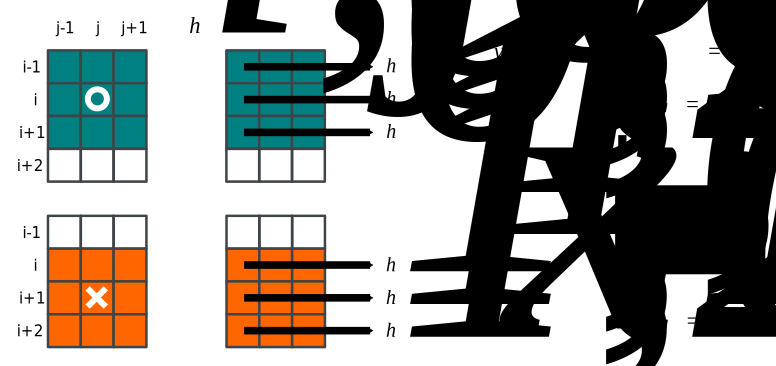
\includegraphics[width=0.55\textwidth]{tiled-conv}
    \caption{Tiled convolution flow}
    \label{pic-tiled-conv}
\end{wrapfigure}


The final step is an optimization published by Advanced Micro Devices (AMD) 
described in \cite{tiled-convolution}. They take advantage from using
separable kernels and reusing operations to get the most out of resources.
We can see separable convolution as a two step process. 
First a horizontal convolution step that creates a set of coefficients 
($h_{y,x}$ in the middle of Fig. \ref{pic-tiled-conv}). Most $h$ coefficients 
are shared by immediate vertical neighbours (e.g. pixels $\hm{\circ}$ 
and $\bm{\times}$ in Fig. \ref{pic-tiled-conv}), thus it is desired 
to reuse them instead of re-computing them. This way, every core in the GPU 
will compute 2 pixels in order to efficiently compute a 2D convolution; plus 
most of this operations are done using registers which is the fastest memory 
available to the cores.


\subsubsection{Comparison}
The Naïve approach seems to be much faster than any other attempts for the 
smallest kernel ($3\times3$), this is simply because a single DoG kernel would
require 9 operations while a separated DoG requires 12. As the size of the
kernels increases tiled convolution has the lead performance-wise.
\begin{table}[hbt]
    \begin{center}
        \caption{Time comparison of different convolution algorithms.}
        \bgroup
        \def\arraystretch{1.2}
        \begin{tabular}{|c|c|c|c|c|}
            \hline Algorithm & Midget Off-centre & Midget On-centre & Parasol Off-centre & Parasol On-centre \\
            \hline Naïve     & 0.000932 s & 0.003150 s & 0.058797 s & N/A\footnote{Unable to fit kernel into constant memory.} \\ 
            \hline Separated & 0.002953 s & 0.005550 s & 0.017261 s & 0.047226 s \\ 
            \hline Tiled     & 0.001947 s & 0.002722 s &  & \\ 
            \hline 
        \end{tabular} 
        \egroup
    \end{center}
\end{table}
\vspace*{-20pt}

For the final implementation we take the best times for every \emph{cell type}
and combine them into a ``convolution'' object under the Python programming language.
%\subsection{Lateral inhibition}
%\label{sec-reconstruction}
%Redundancy is present in biology to ensure robustness of the
system. Nature has developed systems with little data transmission
redundancy. A way to reduce redundancy is through lateral 
inhibition.
\subsubsection{Filter overlap correction algorithm (FoCal)}
\begin{wrapfigure}{r}{0.45\textwidth}
    \vspace{-26pt}
    \begin{minipage}{0.4\textwidth}
        \begin{pseudocode}{FoCal}{coefficients \; S,\\ 
                                  \hspace*{40mm} correlations\; K}
            \label{code-focal}
            P \GETS \emptyset \\
            \WHILE S \neq \emptyset \DO index \GETS max(S), \; value \GETS val(S, index)\\
            \hspace{0.7cm} remove(index, S)\\
            \hspace{0.7cm} append(P, index, value)\\
            \hspace{0.7cm} \FOREACH c \in K \neq 0\\
            \hspace{1.4cm} \FOREACH p \in near\_pixels(index, S) \\
            \hspace{2.1cm}   S(p) \GETS p \; - \; c*value\\
            \RETURN {P}\\
        \end{pseudocode}
            \vspace{-26pt}
    \end{minipage}
\end{wrapfigure}

Neighbouring pixels may contain very similar information;
this redundancy is dealt in the eye, prior to ganglion 
cell spiking, with a mechanism known
as lateral inhibition. In \cite{basab-model},
\citeauthor{basab-model} present an algorithm that
simulates this behaviour, this 
process is done after all ganglion cells have been simulated. 
We shall treat the biggest value as the one to spike first,
then adjust spatially near pixels (in every resulting image)
with the correlation of the kernels in different images 
(Algorithm \ref{code-focal}).
This process is repeated until we run out of pixels with 
positive values and list $P$ is full of corrected coefficients.

%\subsection{Reconstruction via pseudo-inverse}
\subsubsection{Reconstruction procedure}
Spikes are obtained using a \emph{quasi-orthogonal} transformation,
thus reconstruction is a matter of applying the same operation
to every spike generated and to add them up to obtain an approximate
version of the original image (Fig. \ref{pic-original-lena}). If no
lateral inhibition is simulated, the resulting picture is similar to
the original but has redundant information all over the place as seen
in Fig. \ref{pic-unfiltered-spikes}. After correcting for redundancy
the resulting reconstruction is much better, in fact with just 30\% 
of the spikes we can obtain almost a 100 \% of the visual information\cite{basab-model}.

\begin{figure}[hbt]
    \centering
    \begin{subfigure}[t]{0.15\textwidth}
        \centering
        \captionsetup{justification=centering,margin=0.1cm}
        \includegraphics[width=\textwidth]{./Lena-gray}
        \caption{\\Original image}
        \label{pic-original-lena}
    \end{subfigure}
    \begin{subfigure}[t]{0.15\textwidth}
        \centering
        \captionsetup{justification=centering,margin=0.1cm}
        \includegraphics[width=\textwidth]{./final_results-unfiltered}
        \caption{\\100\% raw spikes}
        \label{pic-unfiltered-spikes}
    \end{subfigure}
    %        \hfill
    \begin{subfigure}[t]{0.15\textwidth}
        \centering
        \captionsetup{justification=centering,margin=0.1cm}
        \includegraphics[width=\textwidth]{./final_results-focal-100}
        \caption{\\100\% \emph{corrected} spikes}
        \label{pic-100pc-spikes}
    \end{subfigure}
    \begin{subfigure}[t]{0.15\textwidth}
        \centering
        \captionsetup{justification=centering,margin=0.1cm}
        \includegraphics[width=\textwidth]{./final_results-focal-30pc}
        \caption{\\30\% of \emph{corrected} spikes}
        \label{pic-30pc-spikes}
    \end{subfigure}
    \caption{Results of reconstruction procedure}
\end{figure}
%\clearpage



\section{Project Plan}
\label{sec-project-plan}
The project plan is presented on the following Gantt chart.
%\clearpage
%{
%\color{white}
%\transparent{0.0}
%\lipsum[5-9]
%}


%\begin{wrapfigure}{l}{.5\textwidth}
\begin{figure}[t]
%  \begin{center}

    \hspace*{10cm}
    \begin{rotate}{270}
      \hspace*{1cm}
      \begin{ganttchart}[x unit = 5mm,
                         y unit chart = 5.6mm,
                         vgrid={*1{themecolor, dotted}},
                         compress calendar, 
                         time slot format=isodate-yearmonth,
                         title/.append style={draw=none, fill=themecolordark},
                         title label font=\sffamily\bfseries\color{white},
                         title label node/.append style={below=-1.6ex},
                         title left shift=.05,
                         title right shift=-.05,
                         title height=1]{2014-09}{2017-08}
        \gantttitlecalendar{year, month} \\
         \ganttbar{Learn background concepts}{2014-09}{2015-02}\\
         \ganttbar{Implement retinal models}{2014-12}{2015-04}\\
         \ganttbar{Familiarize with SpiNNaker}{2015-01}{2015-08}\\
         \ganttbar{Develop learning algorithms}{2015-07}{2016-04}\\
         \ganttbar{Develop classification networks}{2015-10}{2016-08}\\
         \ganttbar{Develop vision algorithms}{2016-08}{2017-04}\\
         \ganttbar{Theses writing}{2016-10}{2017-08}\\
      \end{ganttchart}

    \end{rotate}
    \label{fig-project-plan}
%  \end{center}

\end{figure}
%\end{wrapfigure}
%\clearpage
%\vspace*{20cm}

%\lipsum
%\end{multicols}

\end{document}
